% !Mode:: "TeX:UTF-8"

Neste capítulo serão apresentadas as funcionalidades disponíveis ao administrador após a instalação do sistema, referentes ao registro de operadores e gerenciamento das funções disponíveis no sistema.

A parte do administrador é destinada à criação de operadores, cadastro de MSCs e configuração dos modelos de LCR e certificado, bem como à gerência dos certificados emitidos e revogados e suas respectivas estatísticas por tempo e organização. O administrador é também o responsável por exportar e conferir os logs do sistema.

Ao logar como administrador é possível visualizar as tarefas pendentes.

\section{Operadores}\label{sec:operadores}

Ao logar-se como administrador, é possível ver o menu de funções. Ao clicar em \textit{Operadores}, duas possibilidades serão mostradas: \textit{Listar} e \textit{Registrar}.


\subsection{Registrar operadores}\label{subsec:cadEntidades}

Os passos para registrar um operador são simples. Basta selecionar a opção \textit{Registrar} no menu \textit{Operador}. Será carregada uma página, como mostra a figura \ref{fig:registroop}.

\begin{figure}[ht]
     \centering
     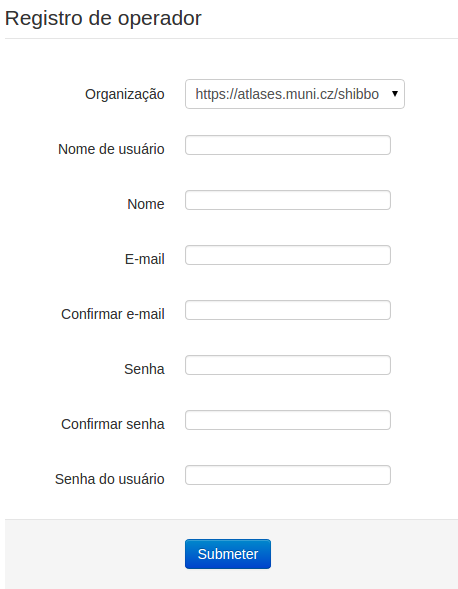
\includegraphics[scale=0.6]{images/registroop.png}
     \caption{Registro de Operador}
     \label{fig:registroop}
\end{figure}

Os campos abaixo devem ser preenchidos com os dados do Operador que está sendo cadastrado:

\begin{itemize}

	\item \textbf{Organização:} Selecione a organização a qual o operador está afiliado;
	\item \textbf{Nome de usuário:} Preencha o nome que o operador deverá utilizar para logar no sistema;
	\item \textbf{Nome:} Preencha o nome completo do operador;
	\item \textbf{E-mail:} Preencha este campo com o respectivo e-mail do operador e repita-o no campo seguinte;
	\item \textbf{Senha:} Escolha uma senha que o operador deverá utilizar para logar no sistema e confirme-a no campo seguinte;
	\item \textbf{Senha do usuário:} Insira a sua senha de administrador para confirmar a operação.
	
\end{itemize}

\subsection{Listar Operadores}

No menu \textit{Operadores $>$ Listar}, o usuário é capaz de visualizar os operadores já cadastrados.
Na página aparecerá uma lista com todos os operadores, semelhante à imagem \ref{fig:listarop}.
Na aba onde são listados é possível ver \textit{Nome de usuário, Nome, Email, Organização e Ação} de cada operador registrado. As ações possíveis são:

\begin{itemize}

	\item \textbf{Excluir operador(}\begin{wrapfigure} 
\includegraphics[height=10]{images/iconedelete2} \end{wrapfigure} \textbf{):} Remove o operador do banco. O mesmo não poderá mais logar no sistema.
	\item \textbf{Editar operador(}\begin{wrapfigure} 
\includegraphics[height=10]{images/iconeeditar} \end{wrapfigure} \textbf{):} É mostrada uma tela onde é possível alterar alguns dados do operador.
	
\end{itemize}

\begin{figure}[ht]
     \centering
     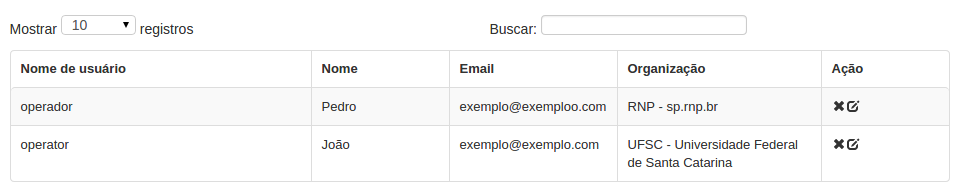
\includegraphics[scale=0.5]{images/listarop.png}
     \caption{Listagem de Operadores}
     \label{fig:listarop}
\end{figure}

\section{SMTP}

\subsection{Registrar SMTP}

SMTP(do inglês \textit{Simple Mail Transfer Protocol}) é o protocolo padrão para envio de e-mails através da Internet. É necessário configurar o e-mail e as mensagens automáticas que devem ser enviadas para o mesmo caso ocorra algum erro ou algum certificado seja emitido.
Para registrar o SMTP deve-se ir ao ícone \textit{SMTP $>$ Registrar}. Será carregada uma página, como mostra a figura \ref{fig:smtp}. É escolha do administrador utilizar uma autenticação extra ou cadastrar sem autenticação (quando não é preciso inserir login e senha do e-mail). 

Caso escolha registrar sem autenticação, siga estes passos:

\begin{itemize}
	\item \textbf{Host Smtp} : Utilizar o IP do servidor SMTP do seu e-mail;
	\item \textbf{E-mail}: E-mail para qual as mensagens devem ser enviadas;
	\item \textbf{Porta}: Se este campo for deixado em branco, será utilizada a porta padrão para as configurações fornecidas. Forçar a utilização de alguma outra porta pode dar problema, por isso forneça uma porta somente se tiver certeza que esta pode ser utilizada com as configurações fornecidas;
    \item \textbf{Tipo de autenticação}: Selecione \textit{Sem autenticação}. Marque a caixa para \textit{Mandar um e-mail teste}. Você deve receber a confirmação do registro de SMTP no e-mail fornecido;
    \item \textbf{Senha do usuário}: Senha do administrador.
\end{itemize}

Caso escolha utilizar algum tipo de autenticação, siga estes passos:

\begin{itemize}
	\item \textbf{Host Smtp} : Utilizar o caminho para o SMTP do seu e-mail. Por exemplo, o caminho para um e-mail do \textit{gmail} seria \textit{smtp.gmail.com};
	\item \textbf{E-mail}: E-mail para qual as mensagens devem ser enviadas;
	\item \textbf{Porta}: Se este campo for deixado em branco, será utilizada a porta padrão para as configurações fornecidas. Forçar a utilização de alguma outra porta pode dar problema, por isso forneça uma porta somente se tiver certeza que esta pode ser utilizada com as configurações fornecidas;
    \item \textbf{Tipo de autenticação}: Selecione \textit{Usuário e Senha}, \textit{Plain} ou \textit{CramMD5}. Marque a caixa para \textit{Mandar um e-mail teste}. Você deve receber a confirmação do registro de SMTP no e-mail fornecido;
    \item \textbf{Protocolo criptográfico}: Selecione \textit{Nenhum}, \textit{SSL} ou \textit{TLS}. Note que alguns servidores de e-mail não aceitam a opção \textit{Nenhum};
    \item \textbf{Nome de usuário}: Informe o login utilizado para entrar no e-mail fornecido;
    \item \textbf{Senha}: Informe a senha utilizada para entrar no e-mail fornecido e confirme-a no campo seguinte;
    \item \textbf{Senha do usuário}: Insira a sua senha de administrador para confirmar a operação.
\end{itemize}

\begin{figure}[ht]
     \centering
     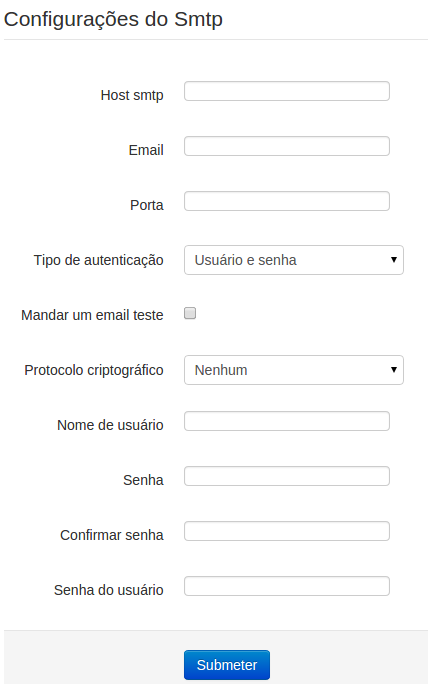
\includegraphics[scale=0.6]{images/smtp.png}
     \caption{Registrar SMTP}
     \label{fig:smtp}
\end{figure}

\subsection{Configurar Mensagens}

Nesta parte do sistema o administrador pode configurar as mensagens que serão enviadas para o seu e-mail de forma automática quando algum evento acontecer. Para configurar as mensagens do SMTP deve-se ir ao ícone \textit{SMTP $>$ Configurar mensagens}. Será carregada uma página, como mostra a figura \ref{fig:msgsmtp}. É possível configurar o assunto e o conteúdo do e-mail para os seguintes eventos:

\begin{itemize}
	\item \textbf{E-mail teste}: É enviado quando um SMTP é registrado com sucesso;
	\item \textbf{Certificado emitido}: É enviado quando um certificado é emitido com sucesso;
	\item \textbf{Erro ao emitir certificado - Sem operadores registrados}: É enviado quando um certificado não pôde ser emitido porque não há nenhum operador registrado no sistema;
	\item \textbf{Erro ao emitir certificado}: É enviado quando ocorre um erro na emissão do certificado;
	\item \textbf{Erro na emissão automática de LCR}: Como será mostrado posteriormente neste manual, é possível configurar a periodicidade em que uma LCR(\textit{Lista de Certificados Revogados}) será emitida. Este tipo de e-mail é enviado quando ocorre um erro nesta emissão automática de LCRs;
	\item \textbf{Erro ao emitir um certificado - Instituição não cadastrada}: É enviado quando um certificado não pôde ser emitido porque não há um operador registrado para a organização que tentou emitir o certificado.
\end{itemize}

\begin{figure}[ht]
     \centering
     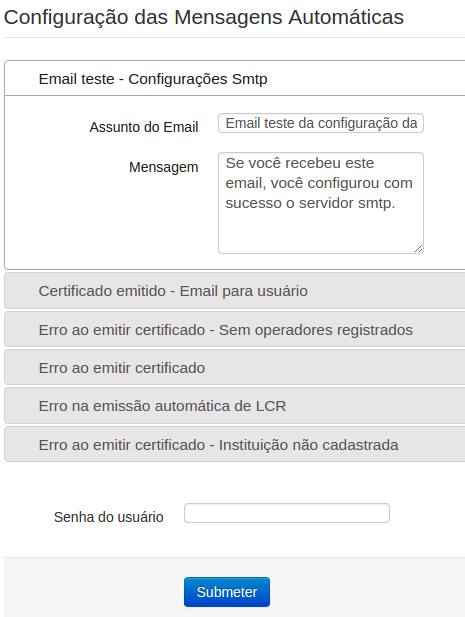
\includegraphics[scale=0.6]{images/msgsmtp.png}
     \caption{Configurar Mensagens}
     \label{fig:msgsmtp}
\end{figure}

\section{Modelos}

Esta é a parte onde deve-se configurar o modelo das LCRs e dos Certificados que serão emitidos.

\subsection{LCR}

Para configurar o template de LCR, basta selecionar o menu \textit{Modelos $>$ LCR}. Aparecerá uma tela igual à imagem \ref{fig:modelolcr} mostrada abaixo. O usuário deve marcar a caixa "Emissão automática" se quiser que a LCR seja emitida de forma automática. Caso não selecione esta opção, deve prosseguir escolhendo logo a baixo a validade da LCR que será emitida, lembrando que só é possível usar uma validade menor que um ano. Deve escolher também o algoritmo que assina a LCR.
Por último deve-se digitar a senha do administrador e clicar no botão \emph{Submeter}.

\begin{figure}[ht]
     \centering
     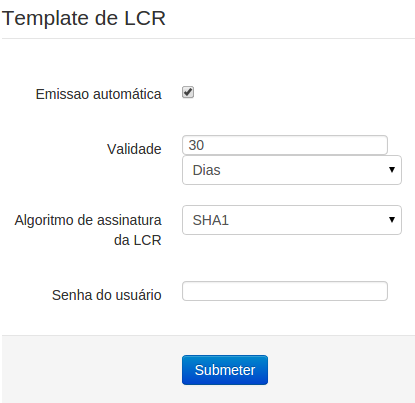
\includegraphics[scale=0.5]{images/modelolcr.png}
     \caption{Modelo de LCR}
     \label{fig:modelolcr}
\end{figure}

\subsection{Certificado}

O administrador deve clicar em \textit{Modelos $>$ Certificado}. Será mostrada uma tela como na figura \ref{fig:modelocert}. É possível configurar vários aspectos do certificado:

\begin{itemize}
	\item \textbf{Uso da chave}: Algumas opções já vêm marcadas por default, mas o administrador pode desmarcá-las se assim desejar. Marque/desmarque o que for desejado e prossiga para a próxima etapa da configuração;
	\item \textbf{Uso extendido da chave}: Nesta etapa, as duas opções disponíveis vêm marcadas por default. Desmarque se for necessário, ou prossiga para a próxima etapa;
	\item \textbf{Políticas de certificado}: Insira os identificadores da Política do Certificado e da Declaração de Práticas de Certificação, se existir;
	\item \textbf{Identificadores da chave}: Os dois identificadores da chave estão marcados por default. Desmarque se for necessário, ou prossiga para a próxima etapa;
	\item \textbf{Validade}: Informe a validade do certificado em dias. Lembrando que esta deve ser um número inteiro de 1 a 3650;
	\item \textbf{Algoritmo de Hash}: Escolha algoritmo que vai assinar o certificado;
	\item \textbf{Odem do serial}: Escolha se deseja que a ordem seja sequencial ou aleatória;
	\item \textbf{Senha do usuário}: Informe a senha do administrador e clique no botão \emph{Submeter}.
\end{itemize}

\begin{figure}[ht]
     \centering
     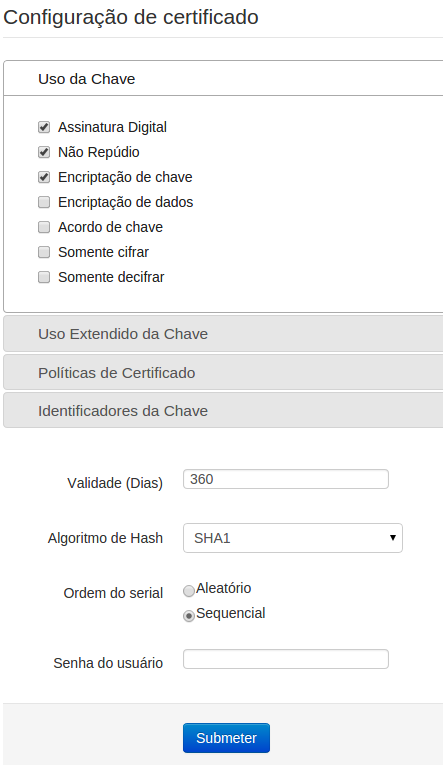
\includegraphics[scale=0.5]{images/modelocert.png}
     \caption{Modelo de Certificado}
     \label{fig:modelocert}
\end{figure}

\section{LCR}

Esta é a parte do sistema que permite que o administrador emita uma Lista de Certificados Revogados até o momento e faça o Download da LCR que desejar.

\subsection{Emitir}

Para emitir uma LCR é preciso acessar o menu \textit{LCR $>$ Emitir}. Basta informar a senha de administrador e clicar \emph{Submeter}. O sistema vai emitir uma lista com todos os certificados revogados até o momento.

\subsection{Download}

Para fazer o download de uma LCR é preciso acessar o menu \textit{LCR $>$ Download}. É possível fazer download de duas formas diferentes, como mostra a figura \ref{fig:lcr}. Se desejar ver as LCRs emitidas em um período específico de tempo, escolha a data de início e fim e clique no botão \emph{Ver LCRs}. Caso deseje ver apenas a última LCR emitida, deixa os campos de início e fim vazios e clique no botão \emph{Baixar a última LCR}.

\begin{figure}[ht]
     \centering
     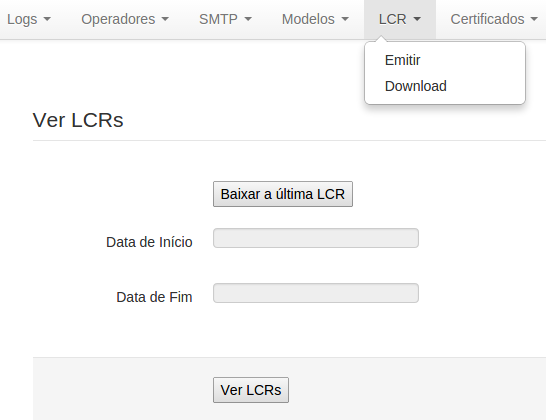
\includegraphics[scale=0.6]{images/lcr.png}
     \caption{Download de LCR}
     \label{fig:lcr}
\end{figure}

\section{Certificados}

No menu \textit{Certificados} é possível listar todos os certificados emitidos até o momento, estejam eles ativos ou revogados. Acesse o menu \textit{Certificados $>$ Listar}. Aparecerá uma tela como mostra a figura \ref{fig:listarcert}. Nesta página é possível ver a organização e o e-mail do operador afiliado à organização responsável pela emissão do certificado, a data em que foi emitido e a data em que este irá expirar e o estado em que se encontra (Ativo ou revogado).
É possível realizar as seguintes ações:

\begin{itemize}

	\item \textbf{Download do certificado(}\begin{wrapfigure} 
\includegraphics[height=10]{images/iconedownload} \end{wrapfigure} \textbf{):} Ao clicar nesse ícone você faz o download do certificado selecionado.
	\item \textbf{Revogar certificado(}\begin{wrapfigure} 
\includegraphics[height=10]{images/iconedelete2} \end{wrapfigure} \textbf{):} Quando um certificado estiver ativo, este ícone irá aparecer na linha do respectivo certificado para que este possa ser revogado individualmente. Se houver necessidade de revogar mais certificados, é possível selecioná-los e revogalos de uma só vez através do ícone de revogação no canto inferior direito da imagem. 
	
\end{itemize}

\begin{figure}[ht]
     \centering
     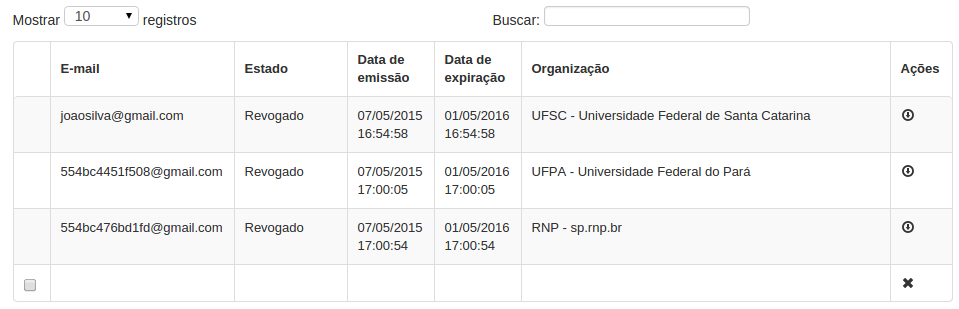
\includegraphics[scale=0.5]{images/listarcert.png}
     \caption{Listagem de certificados}
     \label{fig:listarcert}
\end{figure}

\section{Backup}

Fazer um backup do sistema significa salvar toda a sua estrutura. O backup contém todas as operações realizadas até o momento. O backup do sistema de emissão de certificados ICPEdu é cifrado, pelo fato de poder haver dados sigilosos, a partir de uma senha que será escolhida pelo usuário.

\subsection{Gerar}

Para gerar o backup, basta selecionar o menu \textit{Backup $>$ Gerar}. Aparecerá uma tela igual à imagem \ref{fig:gerarbackup} mostrada abaixo. O usuário deve preencher o primeiro campo com a senha para cifrar o backup e confirmá-la no campo abaixo. É importante armazenar essa senha em local seguro, pois sem ela, será impossível restaurar o backup.
Por último deve-se digitar a senha do usuário e clicar no botão \emph{Submeter}.

\begin{figure}[ht]
     \centering
     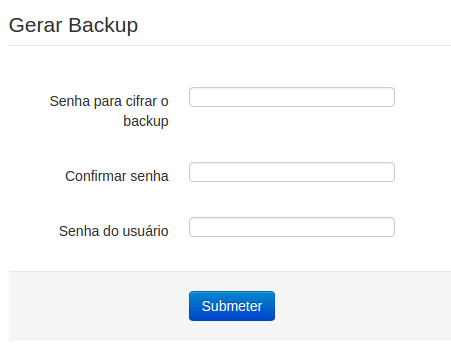
\includegraphics[scale=0.6]{images/gerarbackup.png}
     \caption{Gerar Backup}
     \label{fig:gerarbackup}
\end{figure}

\subsection{Restaurar}

O administrador deve entrar no sistema e clicar em \textit{Backup $>$ Restaurar}. Será mostrada a seguinte tela \ref{fig:restaurarbackup}:

\begin{figure}[ht]
     \centering
     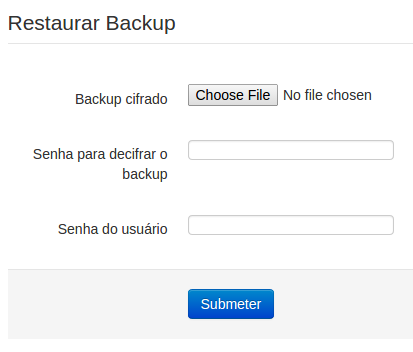
\includegraphics[scale=0.6]{images/restaurarbackup.png}
     \caption{Restaurar Backup}
     \label{fig:restaurarbackup}
\end{figure}

No primeiro campo o usuário deve selecionar o arquivo de backup, gerado e salvo na etapa anterior. Depois deve digitar a senha para decifrar o backup, que deve ser a mesma definida na etapa de geração de backup. Por último, informe a senha do administrador e clique no botão \textit{Submeter}.

\section{Estatísticas}

Esta parte do sistema destina-se à mostrar as estatísticas (por tempo ou por organização) dos certificados emitidos. É possível verificar quantos certificados já foram emitidos e quantos ainda estão ativos. Quando já houver muitos certificados emitidos no sistema, é mais rápido e prático consultar as estatísticas do que contar a quantidade de certificados listados no menu \textit{Certificados}.

\subsection{Total}

Acesse o menu \textit{Estatísticas $>$ Total}. Aparecerá uma tela como mostra a figura \ref{fig:estotal}. É possível ver quantos certificados já foram emitidos no total, bem como quantos ainda estão ativos, quantos já foram revogados e quantos estão expirados. Logo em baixo é possível clicar nas organizações e ver as estatísticas em separado de cada uma delas. Lembrando que, para poder ver a estatística de uma organização específica, é necessário possuir um operador cadastrado para ela, do contrário a organização não aparecerá na tela como mostrado na figura abaixo.

\begin{figure}[ht]
     \centering
     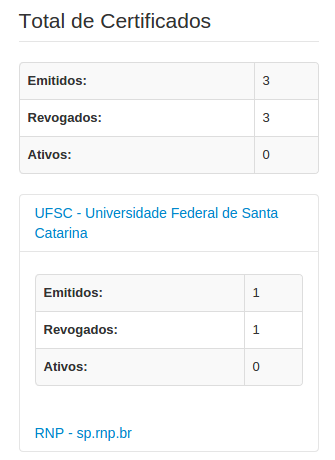
\includegraphics[scale=0.6]{images/estatisticatotal.png}
     \caption{Estatísticas total}
     \label{fig:estotal}
\end{figure}

\subsection{Procurar por tempo}

Acesse o menu \textit{Estatísticas $>$ Procurar por tempo}. Aparecerá uma tela como mostra a figura \ref{fig:estempo}.

\begin{figure}[ht]
     \centering
     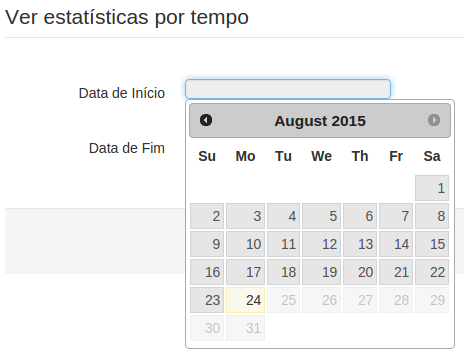
\includegraphics[scale=0.5]{images/estatisticatempo.png}
     \caption{Estatísticas por tempo}
     \label{fig:estempo}
\end{figure}

Para ver a estatística dos certificados emitidos em um período específico de tempo, escolha a data de início e fim e clique no botão \emph{Ver Estatísticas}.

\section{Atributos}

Através do menu \textit{Atributos $>$ Mapeador de atributos} o administrador pode escolher quais atributos o certificado vai requerer, como mostra a figura \ref{fig:atmap}.

\begin{figure}[ht]
     \centering
     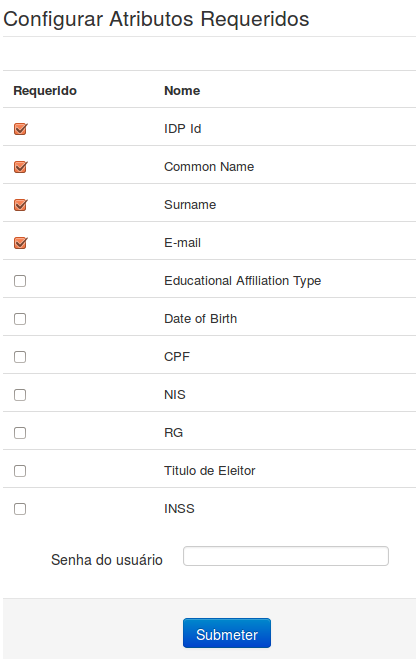
\includegraphics[scale=0.6]{images/attributesmapper.png}
     \caption{Mapeador de atributos}
     \label{fig:atmap}
\end{figure}

Marque os atributos que devem aparecer obrigatoriamente no seu certificado, insira sua senha de administrador e clique no botão \textit{Submeter}.

\section{Cron}

Através do menu \textit{Cron $>$ Tarefas do Cron} é possível verificar as próximas tarefas agendadas para o Cron e também agendar uma nova.

\subsection{Emissão automática de LCR}

Caso o administrador já tenha configurado a periodicidade em que as LCRs devem ser emitidas (pode ser feito através do menu \textit{Modelos $>$ LCR}), será possível verificar sua próxima emissão, sem ser possível alterá-la, como mostra a figura \ref{fig:cron}.

\begin{figure}[ht]
     \centering
     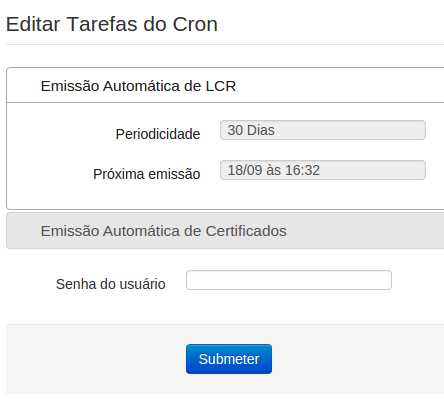
\includegraphics[scale=0.5]{images/cron.png}
     \caption{Emissão automática de LCR}
     \label{fig:cron}
\end{figure}

\subsection{Emissão automática de Certificados}

É possível editar as tarefas do Cron que tratam da parte de certificados. Para fazer isso, basta assinar a caixa \textit{Agendar} e inserir a periodicidade desejada, como mostra a figura \ref{fig:croncert}.

\begin{figure}[ht]
     \centering
     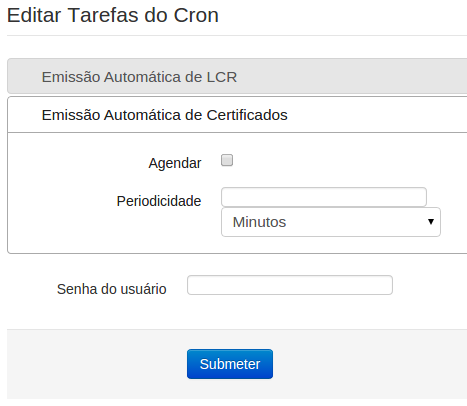
\includegraphics[scale=0.5]{images/croncert.png}
     \caption{Emissão automática de Certificados}
     \label{fig:croncert}
\end{figure}

Insira sua senha de administrador e clique no botão \textit{Submeter}.

\section{Alterar dados do usuário e Sair}

O administrador poder alterar seus dados pessoais e sair do sistema a qualquer momento, basta clicar na engrenagem localizada ao lado superior direito da tela. Duas operações aparecerão: \textit{Alterar dados do usuário} e \textit{Sair}. Ao clicar em \textit{Alterar dados do usuário}, aparecerá uma tela com os campos de dados pessoais, como mostra a figura \ref{fig:alteraadmin}. Altere o que desejar, insira a sua senha de administrador e clique no botão \emph{Submeter}.

\begin{figure}[ht]
    \centering
     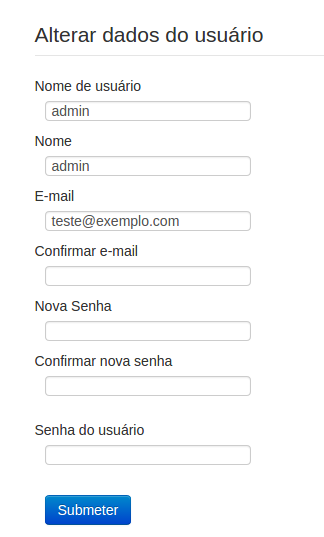
\includegraphics[scale=0.5]{images/alterardadosadmin.png}
     \caption{Alterar dados do usuário}
     \label{fig:alteraadmin}
\end{figure}

\section{Logs}\label{sec:logs}

O administrador pode exportar ou apagar os \textit{logs} do sistema a qualquer momento. Este arquivo contém todas as operações efetuadas pelo sistema de emissão de certificados ICPEdu até o momento em que o \textit{log} tenha sido exportado, em um formato de texto, onde cada ação é uma frase. Para fazer qualquer uma das duas operações, vá ao menu \textit{Logs}, como mostra a figura \ref{fig:logs}.

\begin{figure}[ht]
    \centering
     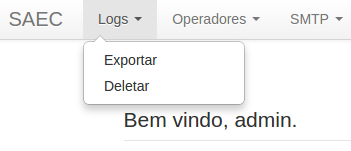
\includegraphics[scale=0.5]{images/logs.png}
     \caption{Menu Logs}
     \label{fig:logs}
\end{figure}

\subsection{Deletar Logs}

Para apagar seus \textit{logs}, basta clicar no menu \textit{Logs $>$ Deletar}. O administrador será direcionado para uma tela que pedirá sua senha para confirmar a ação. 

\subsection{Exportar Logs}

No menu \textit{Logs $>$ Exportar}, pode-se exportar os \textit{logs} do usuário. Ao clicar, o download acontecerá automaticamente. Abra o arquivo e verifique as últimas ações. Caso o \textit{log} tenha sido deletado anteriormente, esta ação deverá estar presente no arquivo.

